\documentclass[12pt,titlepage]{article}
\usepackage[margin=1.25in]{geometry}
\usepackage{graphicx,amsmath,blindtext,minted}

%% Variables definition
\newcommand{\vSubject}{Basic Programming Practicum}
\newcommand{\vSubtitle}{Jobsheet 4 Selection 1}
\newcommand{\vName}{Dicha Zelianivan Arkana}
\newcommand{\vNIM}{2241720002}
\newcommand{\vClass}{1i}
\newcommand{\vDepartment}{Information Technology}
\newcommand{\vStudyProgram}{D4 Informatics Engineering}

%% [START] Tikz related stuff
\usepackage{tikz}
\usetikzlibrary{svg.path,calc,shapes.geometric}
\tikzstyle{terminator} = [rectangle, draw, text centered, rounded corners = 1em, minimum height=2em]
\tikzstyle{process} = [rectangle, draw, text centered, minimum height=2em]
\tikzstyle{decision} = [diamond, draw, text centered, minimum height=2em]
\tikzstyle{data}=[trapezium, draw, text centered, trapezium left angle=60, trapezium right angle=120, minimum height=2em]
\tikzstyle{connector} = [line width=0.5mm,->]
%% [END] Tikz related stuff

%% [START] Fancy header related stuff
\usepackage{fancyhdr}
\pagestyle{fancy}
\setlength{\headheight}{15pt} % compensate fancyhdr style
\fancyhead{}
\fancyfoot{}
\fancyfoot[L]{\thepage}
\fancyfoot[R]{\textit{\vSubject - \vSubtitle}}
\renewcommand{\footrulewidth}{0.4pt}% default is 0pt, overline for footer
%% [END] Fancy header related stuff

%% [START] Custom tabular command related stuff
\usepackage{tabularx}
\newcommand{\details}[2]{
    #1 & #2  \\
}
%% [END] Custom tabular command related stuff

%% [START] Figure related stuff
\newcommand{\image}[3][1]{
    \begin{figure}[h]
        \centering
        \includegraphics[#1]{#2}
        \caption{#3}
        \label{#3}
    \end{figure}
}
%% [END] Figure related stuff

\begin{document}
\begin{titlepage}
    \centering
    \vfill
    {\bfseries\LARGE
        \vSubject\\
        \vskip0.25cm
        \vSubtitle
    }
    \vfill
    
\includegraphics[width=6cm]{images/polinema-logo.png}
    \vfill
    {
        \textbf{Name}\\
        \vName\\
        \vskip0.5cm
        \textbf{NIM}\\
        \vNIM\\
        \vskip0.5cm
        \textbf{Class}\\
        \vClass\\
        \vskip0.5cm
        \textbf{Department}\\
        \vDepartment\\
        \vskip0.5cm
        \textbf{Study Program}\\
        \vStudyProgram
    }
\end{titlepage}

\tableofcontents
\pagebreak

\section{Laboratory}
\subsection{Experiment 1}
\begin{enumerate}
    \item {
        Observe the flowchart

        \begin{figure}[h]
            \centering
            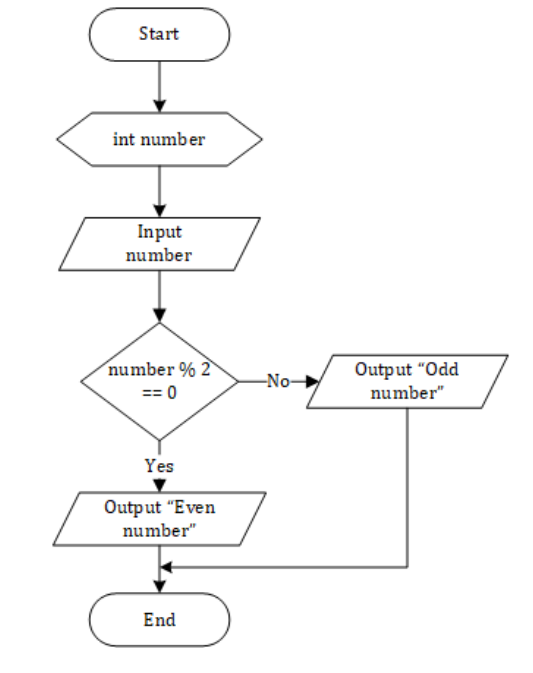
\includegraphics[width=.6\textwidth]{./images/flowchart-1.png}
            \caption{Flowchart}
        \end{figure}

        The flowchart is used to determine odd or even numbers, then we will make the program based on the flowchart.
    }
    \item Open a text editor. Create a new file, name it \textbf{Selection1.java}
    \item Write the basic structure of the Java programming language which contains the \texttt{main()} function
    \item {
        Add the scanner library. Write the following code at the top \textbf{outside the class}

        \begin{minted}[autogobble]{java}
            import java.util.Scanner;
        \end{minted}
    }
    \item {
        Make a scanner declaration. Write the following code in \textbf{in the \texttt{main()}} function

        \begin{minted}[autogobble]{java}
            Scanner input = new Scanner(System.in);
        \end{minted}
    }
    \item {
        Create an \texttt{int} variable with the name \textbf{number}

        \begin{minted}[autogobble]{java}
            int number;
        \end{minted}
    }
    \item {
        Write down the syntax for entering the value from keyboard.

        \begin{minted}[autogobble]{java}
            System.out.print("Enter a number: ");
            number = input.nextInt();
        \end{minted}
    }
    \item {
        Create a selection structure to check whether the number is even or odd

        \begin{minted}[autogobble]{java}
            if (number % 2 == 0) {
                System.out.println("Even number");
            } else {
                System.out.println("Odd number");
            }
        \end{minted}
    }
    \item {
        Compile and run the program. Observe the results!

        \begin{figure}[h]
            \centering
            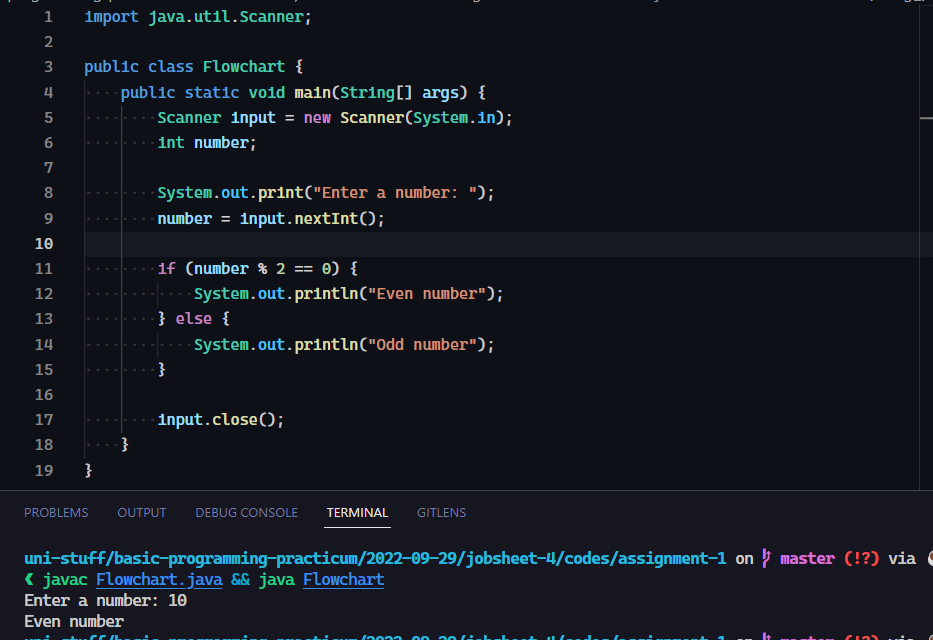
\includegraphics[width=.8\textwidth]{./images/flowchart-impl.png}
            \caption{Implementation according to flowchart}
        \end{figure}
    }
    \pagebreak
\end{enumerate}
\subsection*{Questions}
\begin{enumerate}
    \item {
        Modify the program in its selection structure so that it becomes as follows:

        \begin{minted}[autogobble,fontsize=\small]{java}
            String output = (number % 2 == 0) ? "Even numbers" : "Odd numbers";
            System.out.println(output);
        \end{minted}
    }
    \item {
        Compile, run, and observe the results!

        \begin{figure}[h]
            \centering
            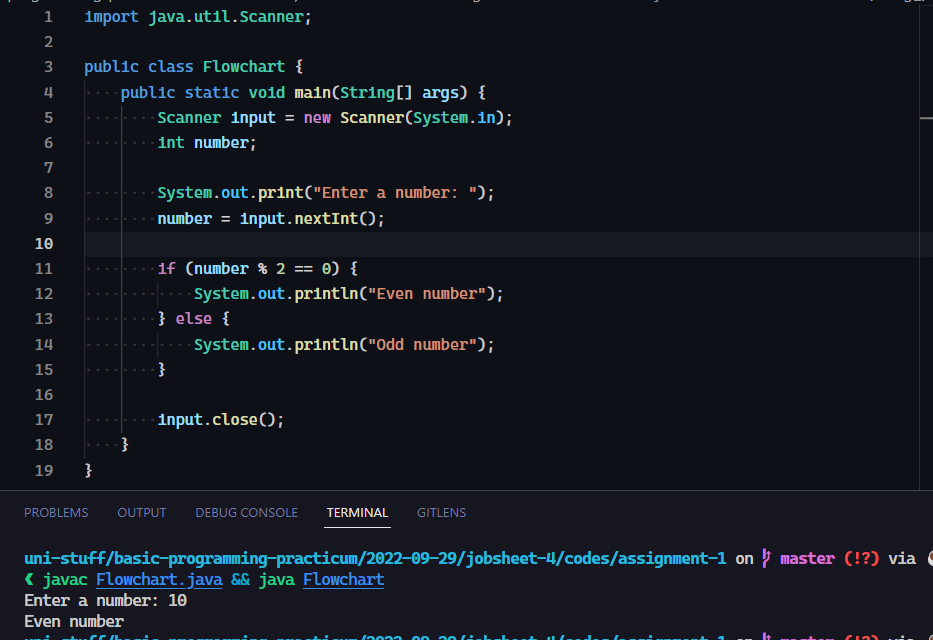
\includegraphics[width=.8\textwidth]{./images/flowchart-impl.png}
            \caption{Implementation with ternary}
        \end{figure}
    }
    \item {
        Explain why the modified program output is the same as the program output before it was modified!

        Because we only replaced the if statement with a ternary but we don't change the condition.
        It will stay \texttt{true} when \texttt{number \% 2 == 0}
    }
\end{enumerate}
\pagebreak
\subsection{Experiment 2}
\begin{enumerate}
    \item Open a text editor. Create a new file, named it \textbf{Selection2.java}
    \item Write the basic structure of the Java programming language which contains the \texttt{main()} function
    \item {
        Add the \textbf{Scanner} library. Write the following code at the top \textbf{outside the class}

        \begin{minted}[autogobble,fontsize=\small]{java}
            Scanner input = new Scanner(System.in);
        \end{minted}
    }
    \item {
        Create an \texttt{int} variable with the name \textbf{score}

        \begin{minted}[autogobble,fontsize=\small]{java}
            int score;
        \end{minted}
    }
    \item {
        Write down the syntax for entering the value from keyboard

        \begin{minted}[autogobble,fontsize=\small]{java}
            System.out.print("Enter a score: ");
            score = input.nextInt();
        \end{minted}
    }
    \item {
        Add the following selection structure

        \begin{minted}[autogobble,fontsize=\small]{java}
            if (score >= 100) {
                score += 10;
            } else {
                score -= 10;
            }
            System.out.println("The final score is " + score);
        \end{minted}
    }
    \pagebreak
    \item {
        Compile and run the program. Observe the results!

        \begin{figure}[h]
            \centering
            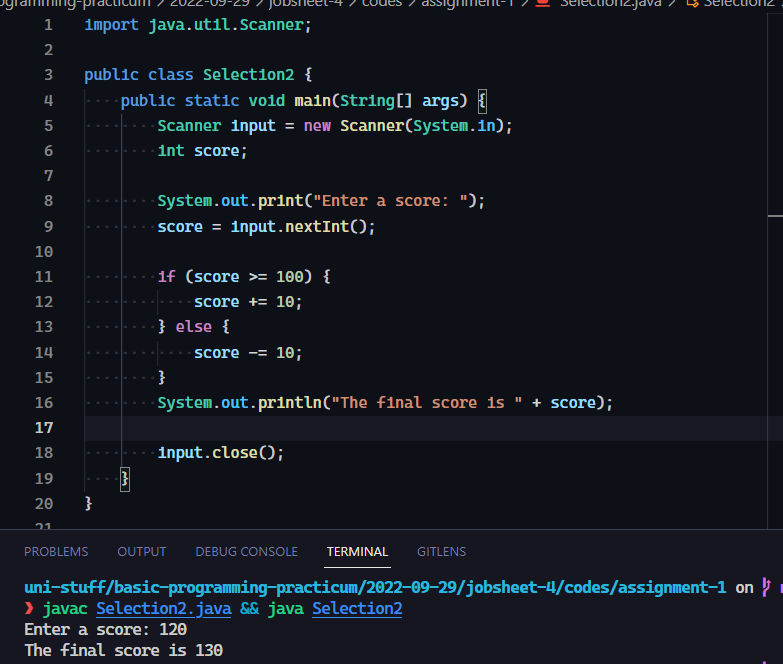
\includegraphics[width=.8\textwidth]{./images/selection-2.png}
            \caption{Selection 2 implementation}
        \end{figure}
    }
\end{enumerate}
\subsection*{Questions}
\begin{enumerate}
    \item {
        Describe the function of the following program code:

        \begin{minted}[autogobble,fontsize=\small]{java}
            score += 10;
            score -= 10;
        \end{minted}

        They are called addition assignment and subtraction assignment. They are used
        to add or subtract and assign the new value add the same time. It is a shorthand
        for doing \texttt{score = score + 10} and \texttt{score = score - 10}
    }
    \pagebreak
    \item {
        Modify the program so that only one input becomes two (for example: \texttt{score1} and \texttt{score2}).
        Then calculate the average of two values, if the average value is more than equal to 100 then subtract 5, whereas
        if the average value is less than 100 it will be printed immediately. 

        \begin{figure}[h]
            \centering
            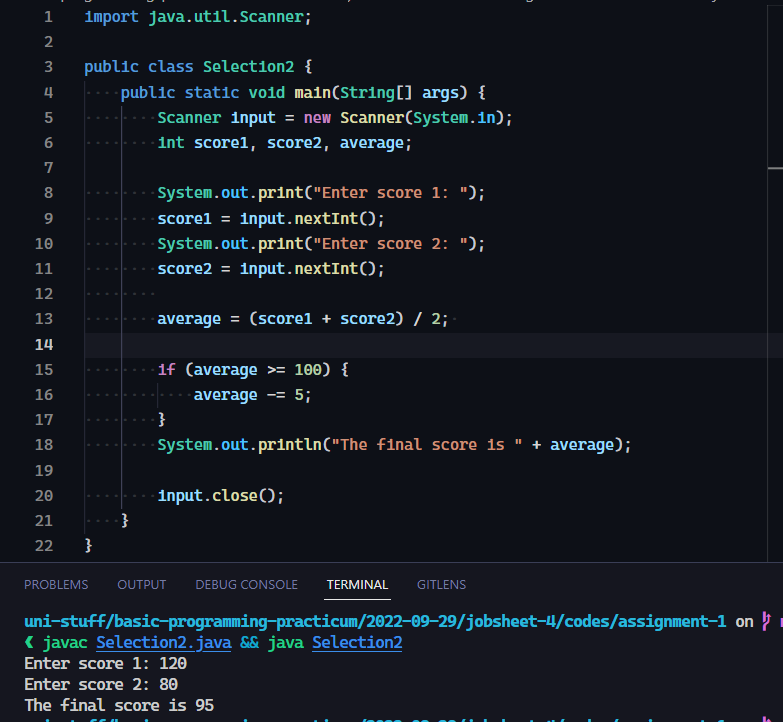
\includegraphics[width=.8\textwidth]{./images/selection-2-average.png}
            \caption{Selection 2 with average}
        \end{figure}
    }
\end{enumerate}
\subsection{Experiment 3}
\begin{enumerate}
    \item Open a text editor. Create a new file. Name it \textbf{Selection3.java}
    \item Write the basic structure of Java programming language which contains the \texttt{main()} function
    \item {
        Add the \textbf{Scanner} library. Write the following code at the top \textbf{outside the class}

        \begin{minted}[autogobble,fontsize=\small]{java}
            import java.util.Scanner;
        \end{minted}
    }
    \item {
        Make a Scanner declaration. Write the following code in the \texttt{main()} function

        \begin{minted}[autogobble,fontsize=\small]{java}
            Scanner input = new Scanner(System.in);
        \end{minted}
    }
    \pagebreak
    \item {
        Create an \texttt{int} variable with the name \texttt{age}

        \begin{minted}[autogobble,fontsize=\small]{java}
            int age;
        \end{minted}
    }
    \item {
        Write down the syntax for entering the value from keyboard:

        \begin{minted}[autogobble,fontsize=\small]{java}
            System.out.print("Enter your age: ");
            age = input.nextInt();
        \end{minted}
    }
    \item {
        Add the following selection structure to check the age category

        \begin{minted}[autogobble,fontsize=\small]{java}
            if (age > 65) {
                System.out.println("Elderly");
            } else if (age > 18) {
                System.out.println("Adults");
            } else if (age > 12) {
                System.out.println("Teen");
            } else if (age > 5) {
                System.out.println("Children");
            } else {
                System.out.println("Toddler");
            }
        \end{minted}
    }
    \pagebreak
    \item {
        Compile and run the program. Observe the results!

        \begin{figure}[h]
            \centering
            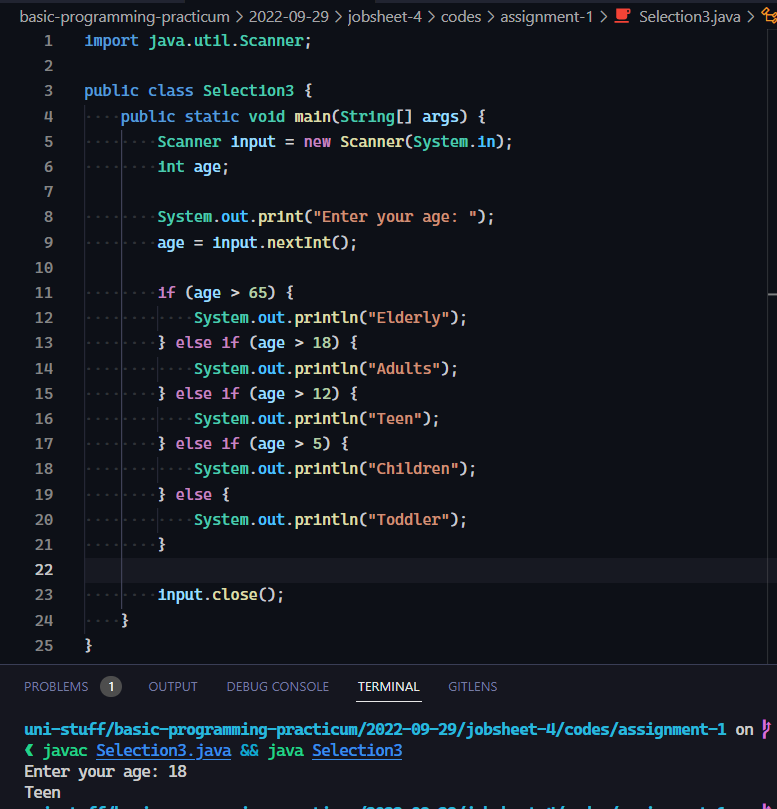
\includegraphics[width=.8\textwidth]{./images/selection-3.png}
            \caption{Selection 3}
        \end{figure}
    }
\end{enumerate}
\subsection*{Questions}
\begin{enumerate}
    \item {
        How many conditions exist in experiment 3? Mention what conditions are!

        There are 5 conditions:
        \begin{itemize}
            \item If the age is greater than 65, then print Elderly
            \item If the age is greater than 18, then print Adults
            \item If the age is greater than 12, then print Teen
            \item if the age is greater than 5, then print Children
            \item Otherwise, print Toddler
        \end{itemize}
    }
    \item {
        Modify the program so that if the age entered is 0 years or less than 0 it will display the output "Sorry, the age you entered is wrong"!

        \begin{figure}[h]
            \centering
            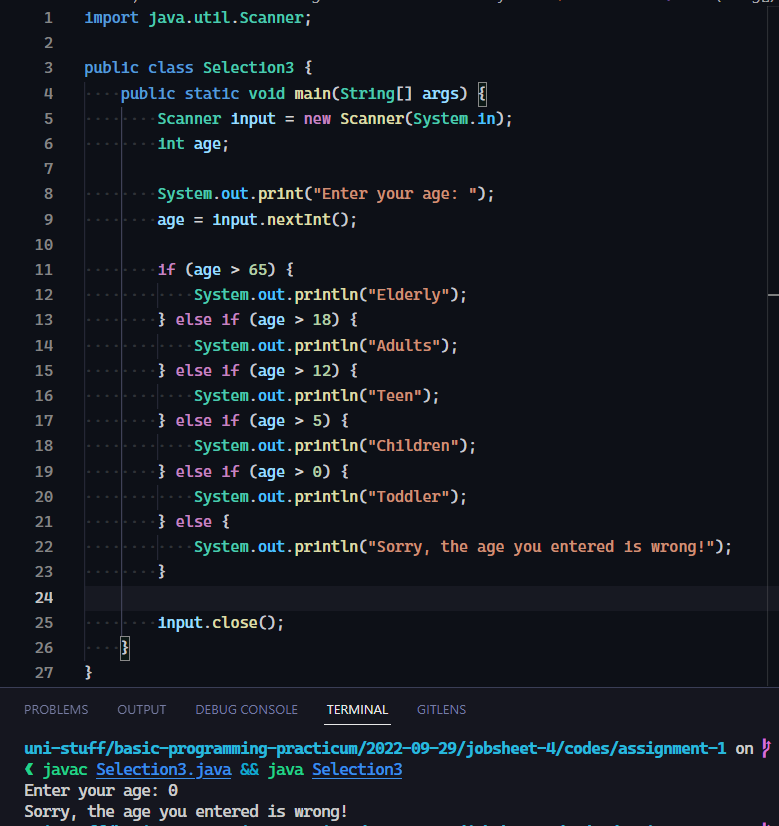
\includegraphics[width=.8\textwidth]{./images/selection-3-zero.png}
            \caption{Selection 3 with less than equal 0 condition}
        \end{figure}
    }
\end{enumerate}
\subsection{Selection4}
\begin{enumerate}
    \item Open a text editor. Create a new file. Name it \textbf{Selection3.java}
    \item Write the basic structure of Java programming language which contains the \texttt{main()} function
    \item {
        Add the \textbf{Scanner} library. Write the following code at the top \textbf{outside the class}

        \begin{minted}[autogobble,fontsize=\small]{java}
            import java.util.Scanner;
        \end{minted}
    }
    \item {
        Make a Scanner declaration. Write the following code in the \texttt{main()} function

        \begin{minted}[autogobble,fontsize=\small]{java}
            Scanner input = new Scanner(System.in);
        \end{minted}
    }
    \item {
        Create the following variables

        \begin{minted}[autogobble,fontsize=\small]{java}
            double number1, number2, result;
            char operator;
        \end{minted}
    }
    \item {
        Write down the syntax for entering values from keyboard

        \begin{minted}[autogobble,fontsize=\small]{java}
            System.out.print("Enter the first number: ");
            number1 = input.nextDouble();
            System.out.print("Enter the second number: ");
            number2 = input.nextDouble();
            System.out.print("Enter an operator (+ - * /): ");
            operator = input.next().charAt(0);
        \end{minted}
    }
    \item {
        Add the following selection structure

        \begin{minted}[autogobble,fontsize=\small]{java}
            switch (operator) {
                case '+':
                    result = number1 + number2;
                    System.out.println(number1 + " + " + number2 + " = " + result);
                    break;
                case '-':
                    result = number1 + number2;
                    System.out.println(number1 + " + " + number2 + " = " + result);
                    break;
                case '*':
                    result = number1 + number2;
                    System.out.println(number1 + " + " + number2 + " = " + result);
                    break;
                case '/':
                    result = number1 + number2;
                    System.out.println(number1 + " + " + number2 + " = " + result);
                    break;
                default:
                    System.out.println("The operator you entered is wrong");
            }
        \end{minted}
    }
    \pagebreak
    \item {
        Compile and run the program. Observe the results!

        \begin{figure}[h]
            \centering
            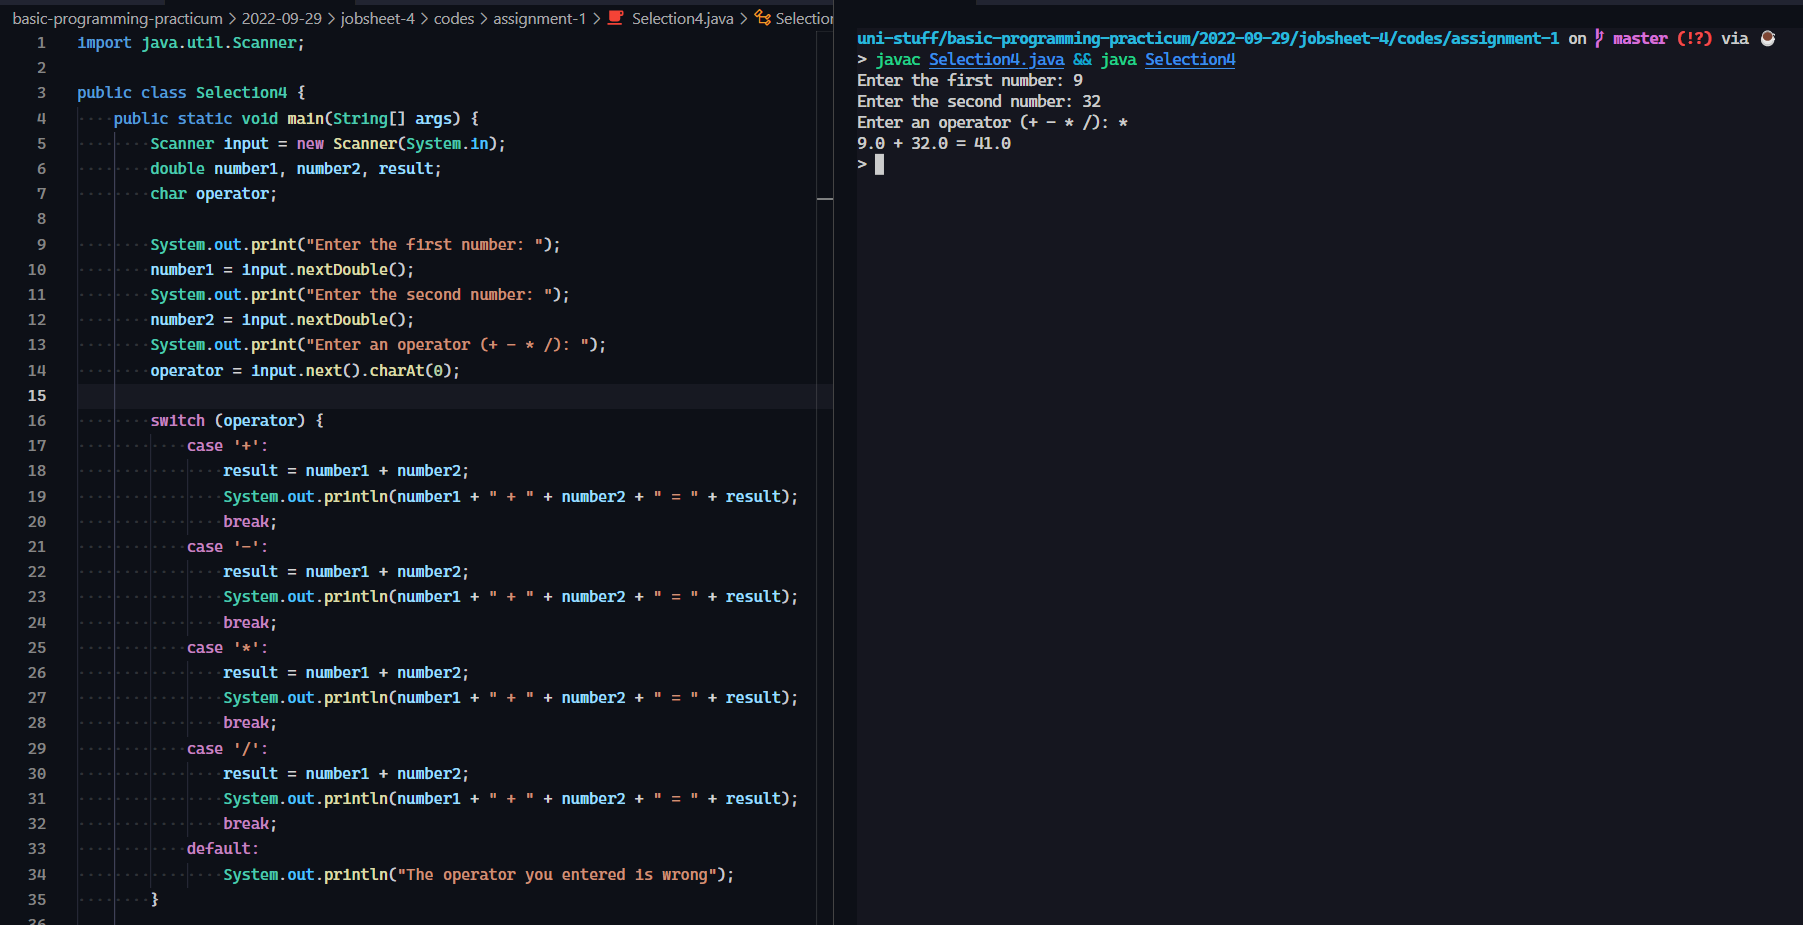
\includegraphics[width=.9\textwidth]{./images/selection-4.png}
            \caption{Selection 4}
        \end{figure}
    }
\end{enumerate}
\subsection*{Questions}
\begin{enumerate}
    \item {
        Explain the function of break and default in experiment 4!

        The \texttt{break} keyword is used to stop the switch statement. If we don't use it, it will just passthrough the next case.
        The \texttt{default} keyword is used as the default condition. It's like an \texttt{else} keyword for a \texttt{switch} statement.
    }
    \item {
        Explain the function of the following program code commands!

        \begin{minted}[autogobble,fontsize=\small]{java}
            operator = input.next().charAt(0);
        \end{minted}

        It is used to get the first character of a String since \texttt{input.next()} will take a String until the next newline.
        In case someone inserted \texttt{*asdasd}, we will only get the \texttt{*} thanks to the \texttt{.charAt(0)} method.
    }
\end{enumerate}
\pagebreak
\section{Assignment}
\begin{enumerate}
    \item {
        Create a program to input two integers, then print on with the largest value!

        \begin{figure}[h]
            \centering
            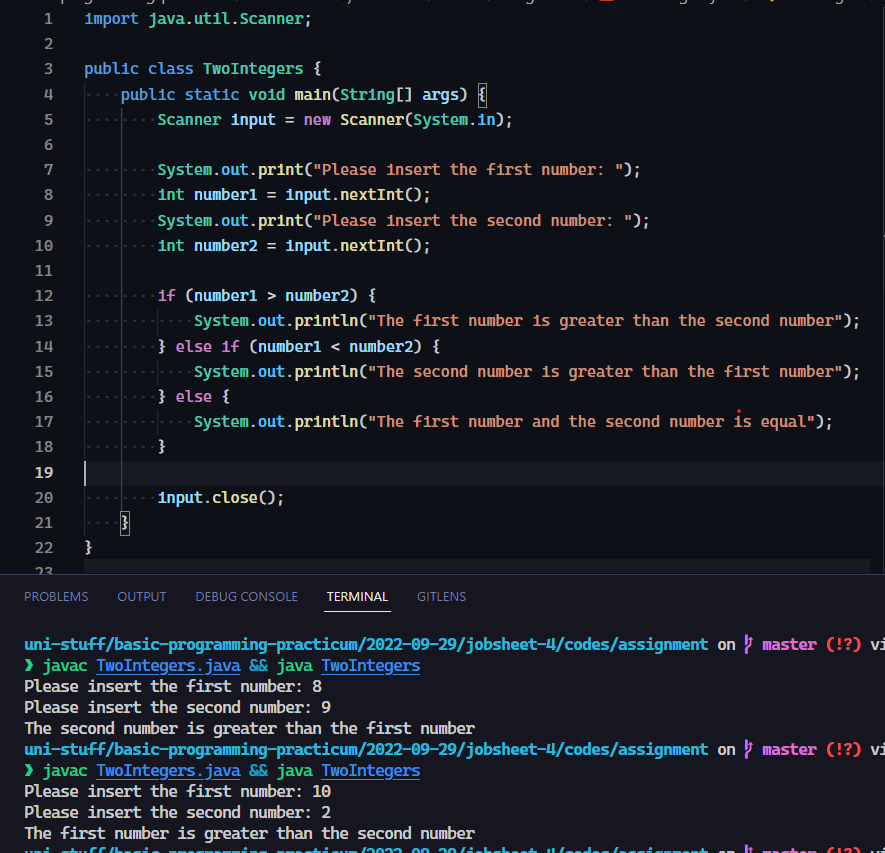
\includegraphics[width=.8\textwidth]{./images/two-integers.png}
            \caption{Comparing two integers}
        \end{figure}
    }
    \pagebreak
    \item {
        Observe the following flowchart!

        \begin{figure}[h]
            \centering
            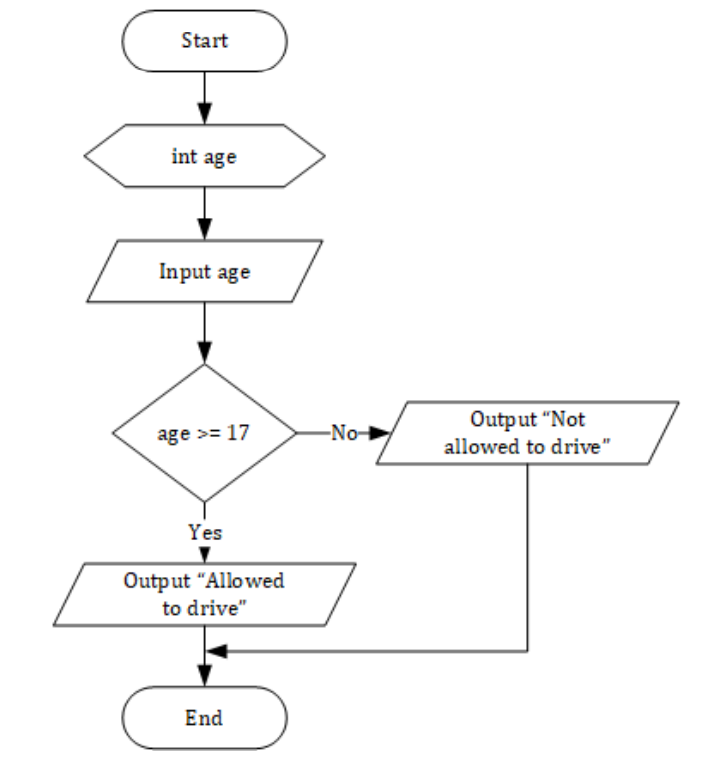
\includegraphics[width=.8\textwidth]{./images/flowchart-2.png}
            \caption{Flowchart}
        \end{figure}

        \pagebreak
        Write program code according to the flowchart!

        \begin{figure}[h]
            \centering
            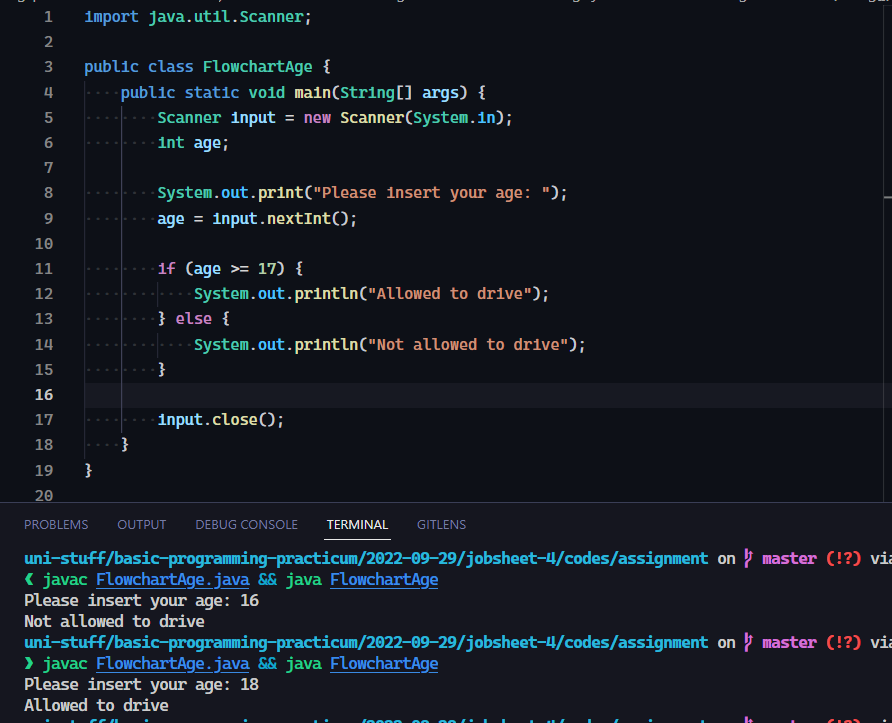
\includegraphics[width=.8\textwidth]{./images/flowchart-age.png}
            \caption{Implementation based on the Flowchart}
        \end{figure}
    }
    \pagebreak
    \item {
        At the end of the semester a lecturer calculates the final score of students which consists of midterm exam score, final exam score, quiz scores, and assignment scores.
        The final score is obtained from 30\% of midterm exams core, 40\% of final exam score, 10\% of quiz scores, and 20\% of assignment scores.
        If the final score of the student is less than 65, then the student will get a remedy.
        Create a program to help determine which students get remedies based on the final score they received!

        \begin{figure}[h]
            \centering
            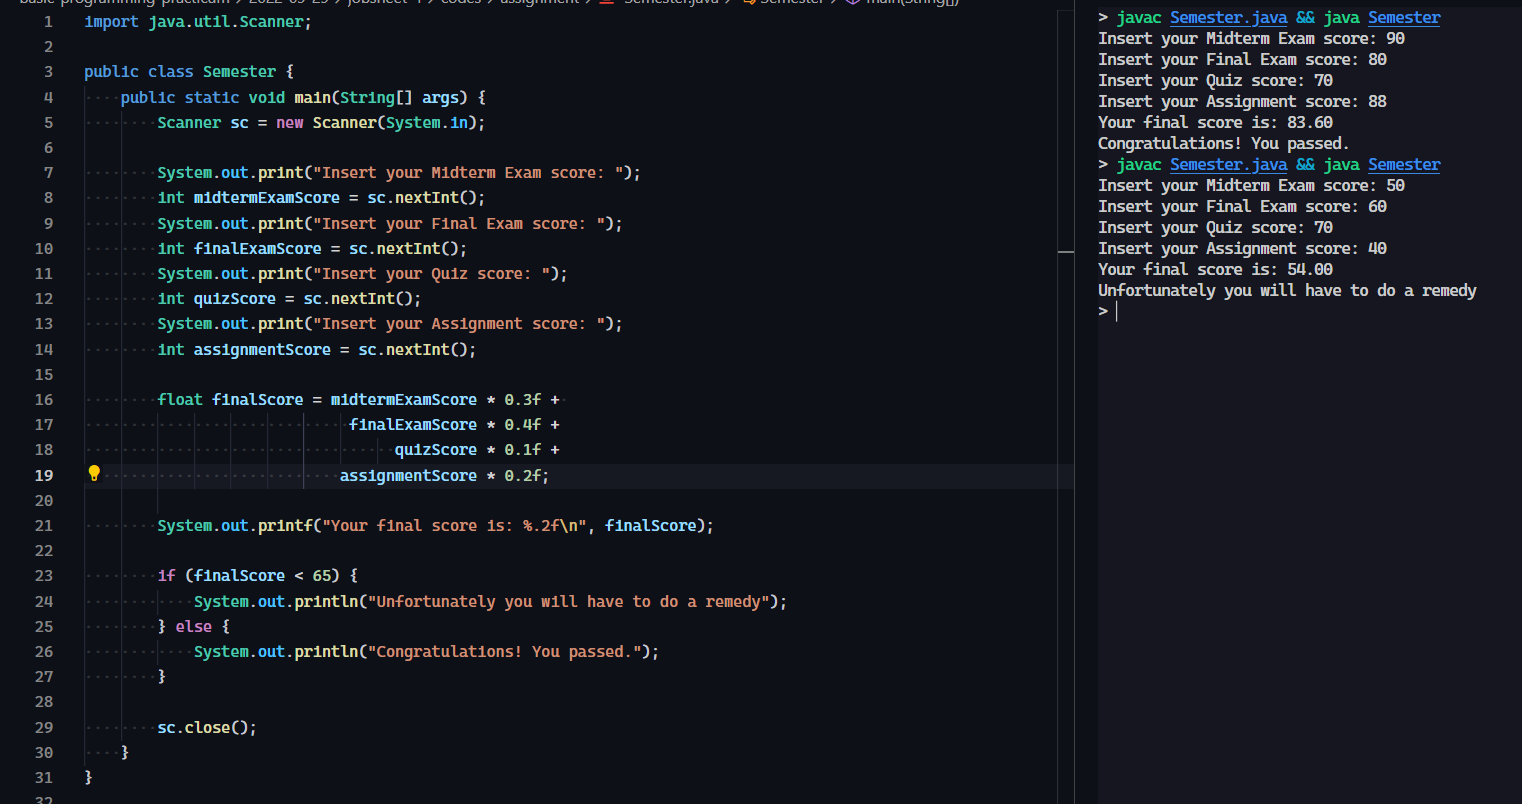
\includegraphics[width=.8\textwidth]{./images/semester.png}
            \caption{Semester score calculation implementation}
        \end{figure}
    }
\end{enumerate}

\end{document}

